
\section{Acquiring Training Data}

As presented in \secref{patter}, for the classification scheme to differentiate between movements, it has to be trained with EMG data from each movement. Training data was acquired using the MYB placed on the forearm while the subject performed the movements: wrist pronation, writst supination, open hand, closed hand and rest. The subsequent section will document how the data used for training the classifier was acquired. \\
First, a baseline recording was made, where the subject was instructed in keeping the hand perfectly still. The baseline consisted of a 15 second recording and was subtracted from each of the other recordings to reduce baseline noise. If the signal was below the baseline amplitude it was set to zero. \\
During a muscle contraction two main states can be recognized; a transient state, described by inconsistent myoelectric activity as the muscle length is changed, and steady state, where a constant firing rate is reached. \cite{Mobarak2014} Classification is often based solely on steady state data, however, including transient state might make for a more robust classifier as the delay until steady state is reached is eliminated \cite{Boschmann2013,Mobarak2014a}. \\
%

\begin{figure}[H]                 
	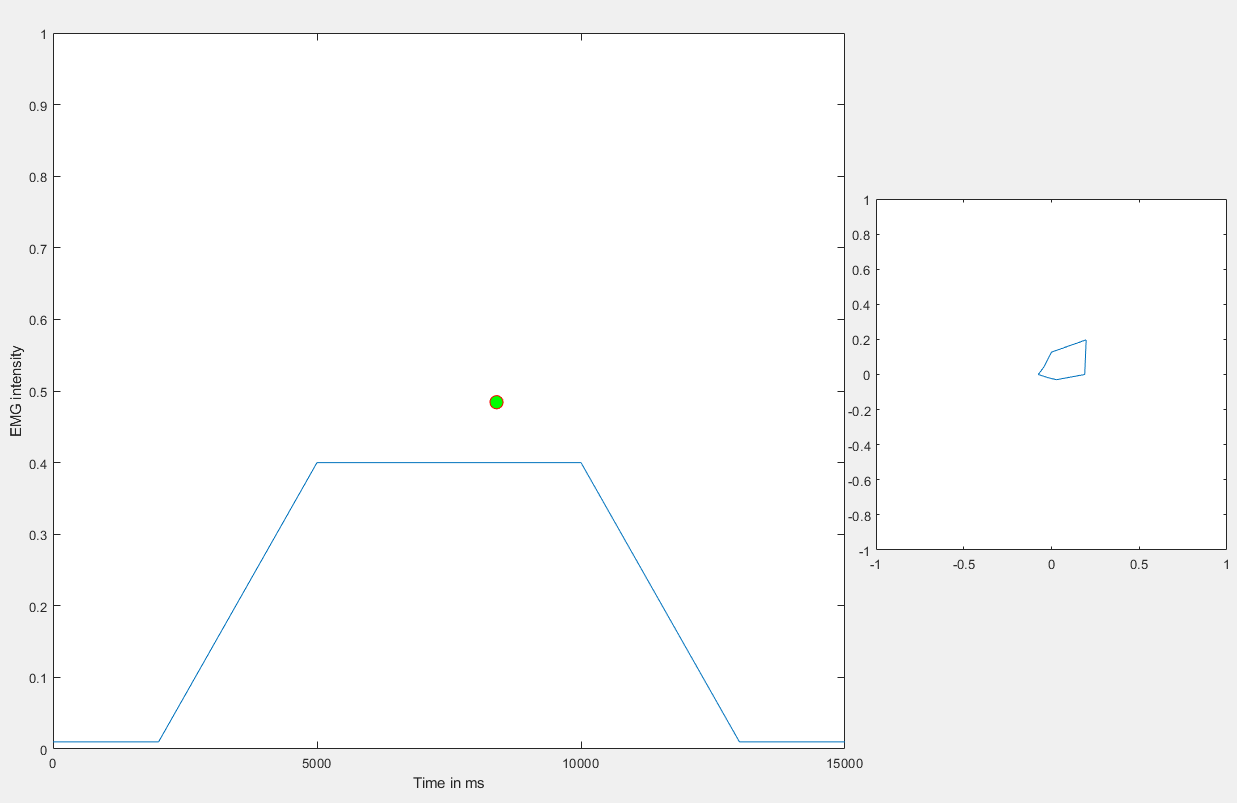
\includegraphics[width=.8\textwidth]{figures/dataacqGUI}  
	\caption{The trapezoidal plot (left) and contraction validation plot (right) used during acquisition of the training data. The line in the trapezoidal plot represented the contraction amplitude requested and the green cursor represented the currently elicited contraction intensity. }
	\label{fig:GUI} 
\end{figure}
\vspace{-1em}

To feed the classifier with training data representing muscle contractions with varying force, different fractions of maximum subject contraction force were recorded. In the process of obtaining training data for each movement the same four were carried out: a maximum voluntary contraction (MVC) recording and a 40 $\percent$, 50 $\percent$ and 70 $\percent$ fraction of MVC recording.
The MVC was recorded for 15 seconds where the subject was instructed to elicit the contraction with a maximum contraction force which could be held steady, without fatigue, over the course of the 15 seconds. This resulted in an MVC for each channel in the MYB. The absolute of the EMG signal for each channel was computed and a mean across all channels was calculated. The mean was used as reference when recording the subsequent training data. \\
Acquisition of the 40 $\percent$, 50 $\percent$ and 70 $\percent$ fraction of MVC were done using a developed graphical user interface (GUI), which can be seen on \figref{fig:GUI}. The image shows the trapezoidal trajectory the subject were instructed to follow using the green cursor, which was a representation of the mean intensity across all channels of the elicited muscle contraction. The cursor would automatically move positively along the x-axis in relation to time. The height of the trapezoid represented either the 40 $\percent$, 50 $\percent$ or 70 $\percent$ fractions of the MVC. Data were recorded during 2.5 seconds rest periods in the beginning and end, a 2.5 incline transition, 5 second steady state and 2.5 second decline transition, summing to a total time of 15 seconds. However, only data recorded during the steady state and the last and first second of the incline and decline transition phase, respectively, were extracted and used to train the classifier. \\
The additional plot seen on the right in \figref{fig:GUI}, plotted the amplitude of each of the eight channels in the MYB and were used by the investigators to assess whether the performed movements were done correctly. If the amplitude of the channels responsible for the performed movement shifted rapidly, or if channels not responsible for the performed movement were active, it would indicate that the subject did not perform a pure contraction and the recording would have to be redone.   
   
   
